\subsection{Berechnung des Trägheitsmoments durch Approximation des Körpers}

\begin{figure}
\begin{minipage}{.49\textwidth}
    \centering
    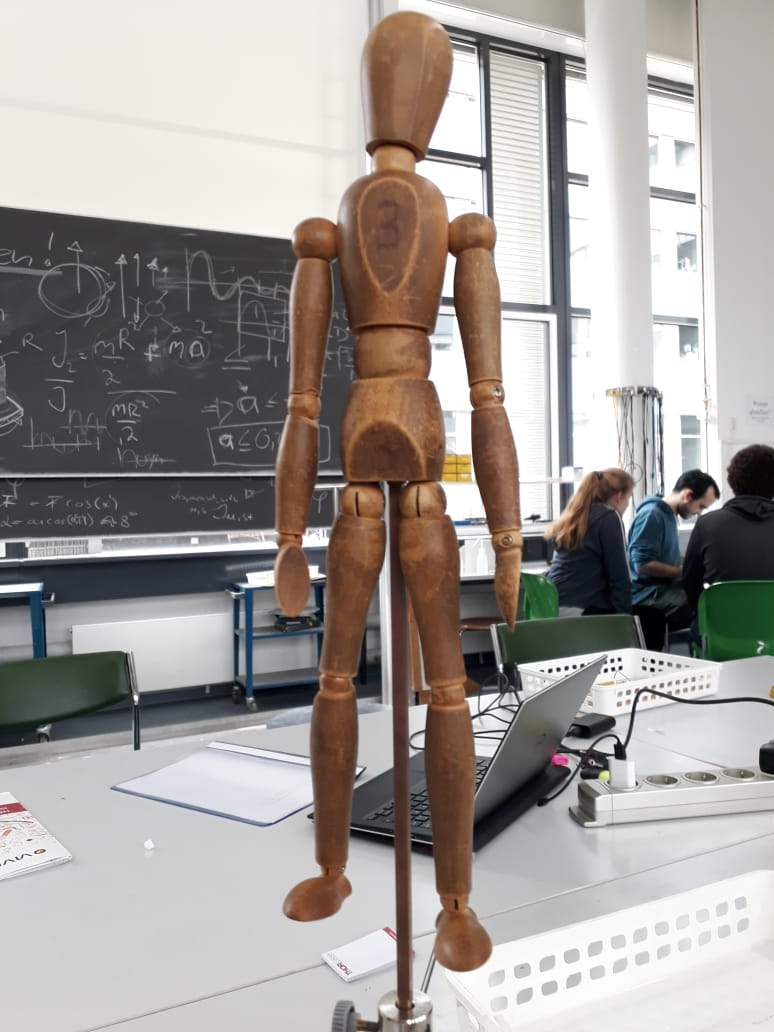
\includegraphics[scale=.28]{./Bilder/figur1.jpeg}
    \caption{Figur 1}
\end{minipage}
\begin{minipage}{.49\textwidth}
    \centering
    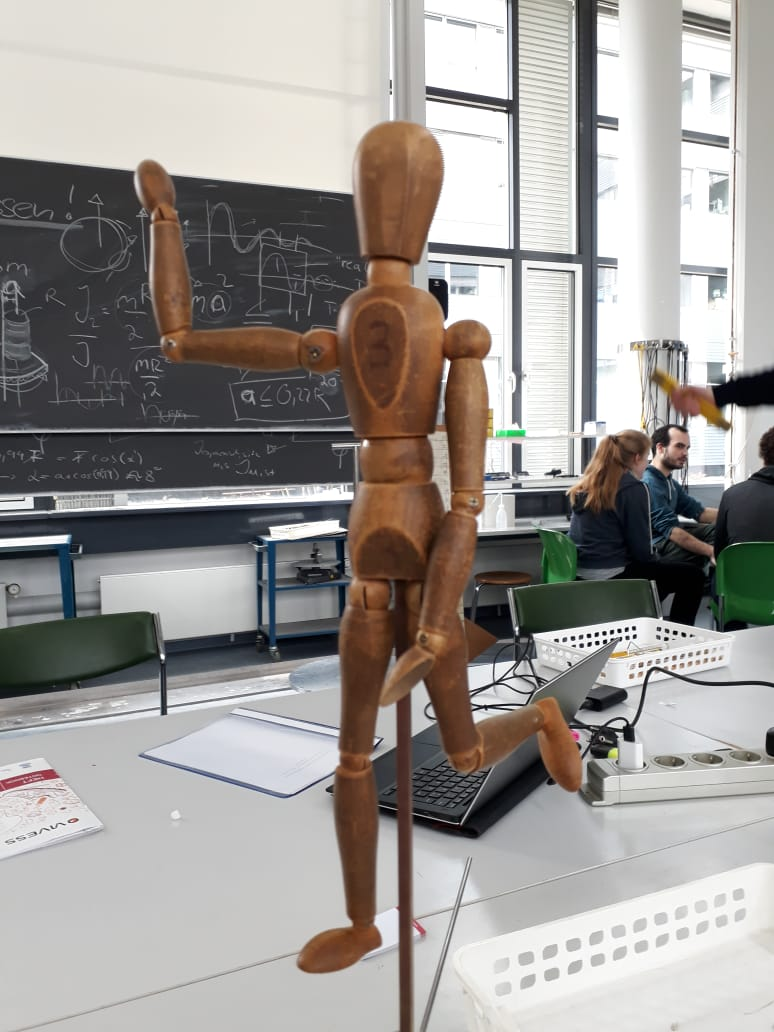
\includegraphics[scale=.28]{./Bilder/figur2.jpeg}
    \caption{Figur 2}
\end{minipage}
\end{figure}


Für Person 1 und Figur 1 errechnen wir ein durch Zylinder und Kugeln genähertes Trägheitsmoment von  $\unit[0.8]{kg\,m^2}$. Für Person 2 und Figur 2 erhalten wir einen Wert von $\unit[1.9]{kg\,m^2}$. 



\begin{table}
\begin{center}
\begin{tabular}{|c|c|c|c|c|c|c|}
\hline 
• & Masse & Höhe & Bein Länge & Bein Radius & Arm Länge & Arm Radius \\
\hline 
Person 1 & 61.4 kg & 185 cm & 94 cm & 6.8 cm & 69 cm & 4.1 cm \\
\hline 
Person 2 & 74.6 kg & 184 cm & 49/60 cm & 6.9 cm & 37/39 cm & 4.9 cm \\
\hline
\end{tabular}
\end{center}

\begin{center}
\begin{tabular}{|c|c|c|c|c|}
\hline
• & Hüfte Höhe & Hüfte Breite & Hüfte Dicke & Kopf Radius \\
\hline
Person 1 & 63 cm & 35 cm & 22 cm & 9.4 cm \\
\hline
Person 2 & 56 cm & 32 cm & 22 cm & 9.4 cm \\ 
\hline
\end{tabular}
\caption{Gemessene Werte für die Annäherung (bei zwei Werten mit ''/'' getrennt ist jeweils Ober-/Unterarm bzw. Ober-/Unterschenkel gemeint)}
\end{center}

\end{table}
